
\newpage
\subsection{Details und Implementation}

\begin{center}
\emph{{\small Sascha Bachmann}}
\end{center}

\bigskip

\noindent Nachdem im vorigen Abschnitt der Marching Cubes Algorithmus allgemein beschrieben wurde, wird im Folgenden auf wichtige Details und auf die konkrete Implementation genauer eingegangen. Der Algorithmus wurde auf Grundlage der Quellen \cite{MC} und \cite{MCADD} implementiert, auf die an geeigneten Stellen noch präziser verwiesen wird.
\medskip

\subsubsection*{Übersicht} Bevor einige Aspekte der Implementation detailliert beschrieben werden, gibt zunächst die folgende Grafik einen Überblick über den Ablauf der Oberflächen-Berechnung.

\noindent
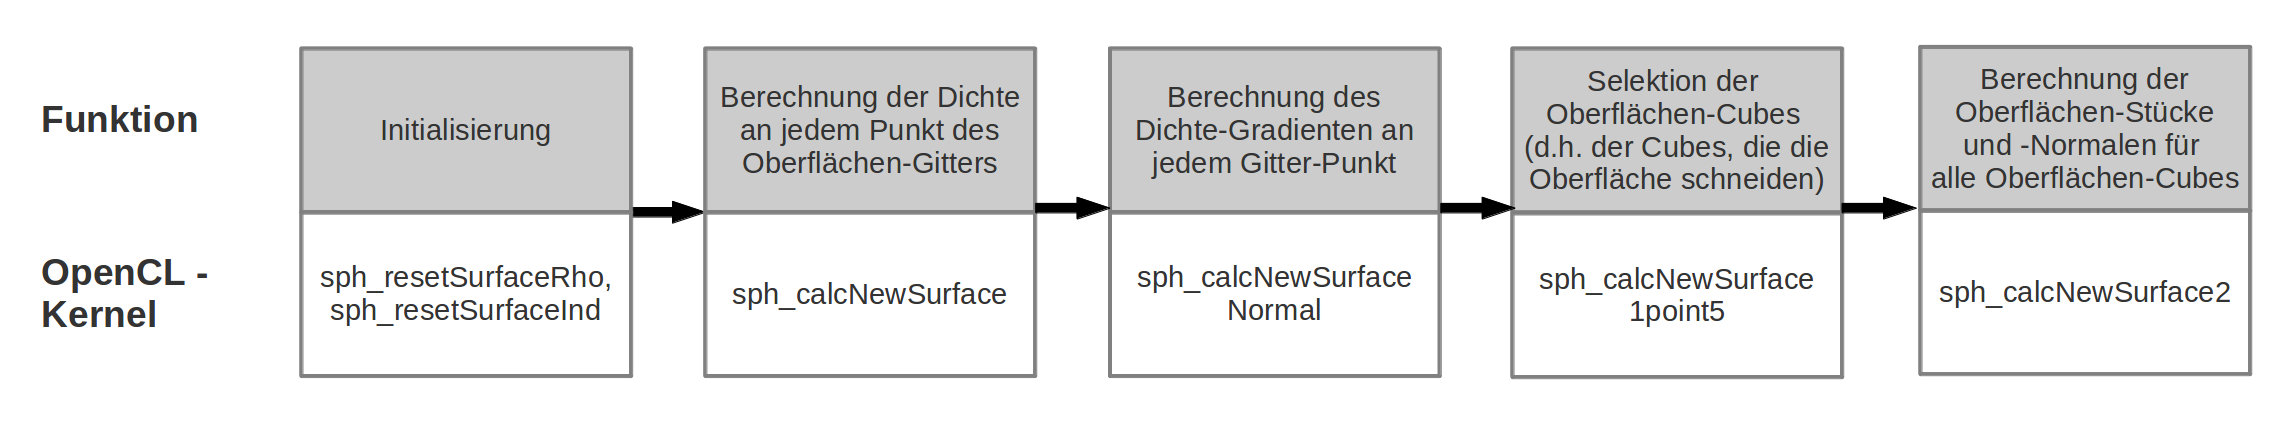
\includegraphics[scale=0.245]{images/MC-Ablauf}
\medskip

\subsubsection*{Berechnung der Gitter-Punkt-Dichten}
Nach der Initialisierung einiger OpenCL-Buffer wird im Kernel {\tt sph\_calcNewSurface} die Dichte an jedem Punkt des Oberflächen-Gitters approximiert. Hierzu wird für jeden Gitter-Punkt $x$ die Dichte $\rho_x$ mittels Gleichung \ref{density} berechnet, also
\begin{align*}
\rho_x = \sum_{i=1}^n m w(x - r_i, h).
\end{align*}
Der naive Ansatz wäre nun, dass je Work-Item sequentiell die obige Summe für einen Gitter-Punkt $x$ berechnet wird. Dies führt allerdings dazu, dass viele Work-Items nichts zu tun haben -- nämlich immer dann, wenn sich der zugehörige Gitter-Punkt außerhalb der Flüssigkeit befindet. Um die Parallelität zu erhöhen hat es sich daher als sinnvoll herausgestellt, für jeden Flüssigkeits-Partikel $i$ ein Work-Item zu starten. In einem OpenCL-Buffer sollen nun für jeden Gitter-Punkt $x$ die Dichten $\rho_x$ abgelegt werden. Hierzu bildet jedes Work-Item die Summanden $m w(x-r_i, h)$ der obigen Dichte-Summe für alle benachbarten Gitter-Punkte $x$ und addiert jeden dieser Summanden mittels der {\tt atomic\_add}-Funktion an die zu $x$ gehörende Stelle des Dichte-Buffers. Es sei noch angemerkt, dass hierbei die Summanden zunächst geeignet skaliert werden, da die {\tt atomic\_add}-Funktion nur Integer-Werte addieren kann.
\medskip
\pagebreak

\subsubsection*{Berechnung der Dichte-Gradienten}
Die Berechnung der Dichte-Gradienten im OpenCL-Kernel {\tt sph\_calcNewSurfaceNormal} erfolgt nach der in \cite[S. 165]{MC} beschriebenen Methode. Jedes Work-Item ist hierbei für die Berechnung des Gradienten an einem der Gitter-Punkte zuständig.
\medskip

\subsubsection*{Selektion der Oberflächen-Cubes}
Nachdem Dichte und Gradienten an den Gitter-Punkten berechnet wurden, kann prinzipiell die Berechnung der Oberflächen-Stücke für jeden Cube des Gitters durchgeführt werden. Hierzu soll sinnvollerweise in einem OpenCL-Kernel für jeden Cube ein Work-Item gestartet werden. Allerdings ist für diejenigen Cubes, die entweder ganz innerhalb oder ganz außerhalb der Flüssigkeit liegen, keine Oberfläche zu berechnen. Bevor daher mit der eigentlichen Oberflächen-Berechnung begonnen wird, werden die Cubes, die tatsächlich von der Oberfläche geschnitten werden, zunächst selektiert. Hierzu wird im Kernel {\tt sph\_calcNewSurface1point5} für jeden Cube des Gittes ein Work-Item gestartet. Jedes Work-Item überprüft nun, ob entweder alle Ecken des Cubes in der Flüssigkeit liegen (d.h. die Dichte an allen Ecken ist größer als ein vorgegebener Schwellenwert) oder ob alle Ecken außerhalb der Flüssigkeit liegen. Tritt einer der beiden Fälle ein, so wird in einem OpenCL-Buffer an der zum betrachteten Cube gehörenden Stelle eine $1$ eingetragen, anderenfalls eine $0$. Anschließend wird dieser Buffer Host-seitig verarbeitet und die Indizes der $0$-Einträge an den Kernel {\tt sph\_calcNewSurface2} übergeben, der für die eigentliche Oberflächen-Berechnung zuständig ist.
\medskip

\subsubsection*{Berechnung der Oberflächen-Stücke und -Normalen}
Zur Berechnung der Oberfläche wird im OpenCL-Kernel {\tt sph\_calcNewSurface2} für jeden zuvor selektierten Oberflächen-Cube ein Work-Item gestartet. Um den Ablauf der Berechnung des Oberflächen-Stückes eines Cubes zu beschreiben, werden zunächst einige Vorbemerkungen benötigt.
\smallskip

\noindent Da jede der acht Ecken eines Cubes entweder in der Flüssigkeit liegt (d.h. die Dichte an diesem Gitter-Punkt übersteigt den Schwellenwert) oder außerhalb, sind zur Bestimmung der richtigen Konfiguration grundsätzlich $2^8 = 256$ Fälle zu unterscheiden. Nummeriert man nun die Ecken mit $1$ bis $8$, so ergibt sich für jeden dieser Fälle ein eindeutiger $8$-Bit-Code, indem das $i$-te Bit genau dann gesetzt wird, wenn die $i$-te Ecke in der Flüssigkeit liegt (vgl. \cite[S. 165]{MC}).
\smallskip

\noindent Mittels diverser Symmetrien (Rotation etc., siehe \cite{MC} und \cite{MCADD} für Details) lassen sich nun die ursprünglichen $256$ Fälle auf einige wenige unterschiedliche Konfigurationen zurückführen. In diesem Projekt werden die Konfigurationen $0$ bis $14$ aus \cite[S. 165]{MC} und zur Vermeidung von Lücken in der Oberfläche ergänzend die Konfigurationen $3a$, $6a$ und $7a$ aus \cite[S. 247]{MCADD} verwendet (letztere erhalten hier die Konfigurations-Nummern $15, 16$ und $17$).
\smallskip
\pagebreak

\noindent Die Zuordnung des 8-Bit-Codes zu einem der insgesamt $18$ unterschiedlichen Konfigurationen wird vor der Simulation in der Java-Klasse {\tt caseMapCreator} berechnet und anschließend in einem constant-Array in den OpenCL-Code geschrieben, welches mit {\tt case\_map} bezeichnet wird. In diesem Array wird für jeden Code zusätzlich zur richtigen Konfigurations-Nummer auch die Permutation der Cube-Ecken abgelegt, die die Ecken der zugeordneten Konfiguration auf die zugehörigen Ecken des ursprünglichen Cubes abbildet.
\smallskip

\noindent Zum Rendern der die Oberfläche darstellenden Dreiecke wird an OpenGL ein Vertex-Buffer und ein Index-Buffer übergeben. Der Vertex-Buffer enthält für jeden Eckpunkt der Oberflächen-Dreiecke sechs Einträge -- die ersten drei geben die räumliche Position des Eckpunktes an und die nächsten drei geben die Oberflächen-Normale an diesem Punkt an. Der Index-Buffer enthält für jedes Oberflächen-Dreieck drei aufeinander folgende Indizes, die sich auf den Vertex-Buffer beziehen und die Eckpunkte des zu zeichnenden Dreiecks festlegen.
\smallskip


\noindent Betrachtet man nun das Oberflächen-Stück eines Oberflächen- Cubes, so liegen die Eckpunkte der Dreiecke, die dieses Stück definieren, genau auf denjenigen Kanten des Cubes, deren eine Ecke innerhalb und deren andere Ecke außerhalb der Flüssigkeit liegt (vgl. \cite[S. 164]{MC}). Jede der $18$ Konfigurationen ist daher genau festgelegt durch die Angabe der beteiligten Kanten für die Eckpunkte und eine Angabe von Indizes, durch die bestimmt ist, welche der Eckpunkte die Dreiecke bilden. Hierzu werden die Kanten des Cubes von $1$ bis $12$ nummeriert. Wie schon die Nummerierung der Ecken folgt auch die in diesem Projekt verwendete Nummerierung der Kanten dem Vorschlag in \cite[S. 165]{MC}. Die Angabe der beteiligten Kanten für jede Konfiguration sowie die Angabe der die Dreiecke definierenden Indizes wird nun in zwei separaten constant-Arrays abgelegt, die mit {\tt confVertex} und {\tt confIndex} bezeichnet werden.
\smallskip


\noindent Wenn nun für einen konkreten Oberflächen-Cube das Oberflächen-Stück berechnet werden soll, so wird zunächst der $8$-Bit-Code berechnet und mittels des {\tt case\_map}-Arrays die richtige Konfigurations-
Nummer bestimmt. Mithilfe dieser Nummer lassen sich aus dem {\tt confIndex}-Array die richtigen Indizes für den OpenGL-Index-Buffer auslesen. Um die richtigen Werte für den OpenGL-Vertex-Buffer zu erhalten, müssen zunächst für jede im {\tt confVertex}-Array hinterlegte Kanten-Nummer die räumliche Position des zugehörigen Dreiecks-Eckpunktes und die Oberflächen-Normale an dieser Stelle berechnet werden. Für jede Kanten-Nummer werden hierzu aus dem constant-Array {\tt edgesToVerts} die zwei zugehörigen Ecken-Nummern ausgelesen. Die Ecken-Nummern werden dann mittels der im {\tt case\_map}-Array hinterlegten Permutation auf die entsprechenden Ecken im ursprünglichen Cube abgebildet. Interpoliert man nun diese ursprünglichen Cube-Ecken mittels der Dichte-Werte an diesen Gitter-Punkten, so erhält man die gewünschte Position des Dreiecks-Eckpunktes und eine analoge Interpolation der zugehörigen Dichte-Gradienten liefert zudem die Normale (vgl. \cite[S. 165]{MC}).
\smallskip

\noindent Abschließend illustriert das folgende Schaubild noch einmal anhand eines Beispiels den Ablauf der Berechnung eines Oberflächen-Stückes. Wie auch bei den Zeichnungen in \cite[S. 165]{MC} werden dabei die in der Flüssigkeit liegenden Cube-Ecken mit schwarzen Punkten gekennzeichnet. Es sei noch angemerkt, dass für die Nummerierung der Cube-Ecken an einigen Stellen die Zahlen $0$ bis $7$ anstatt $1$ bis $8$ verwendet werden.
\medskip

\begin{center}
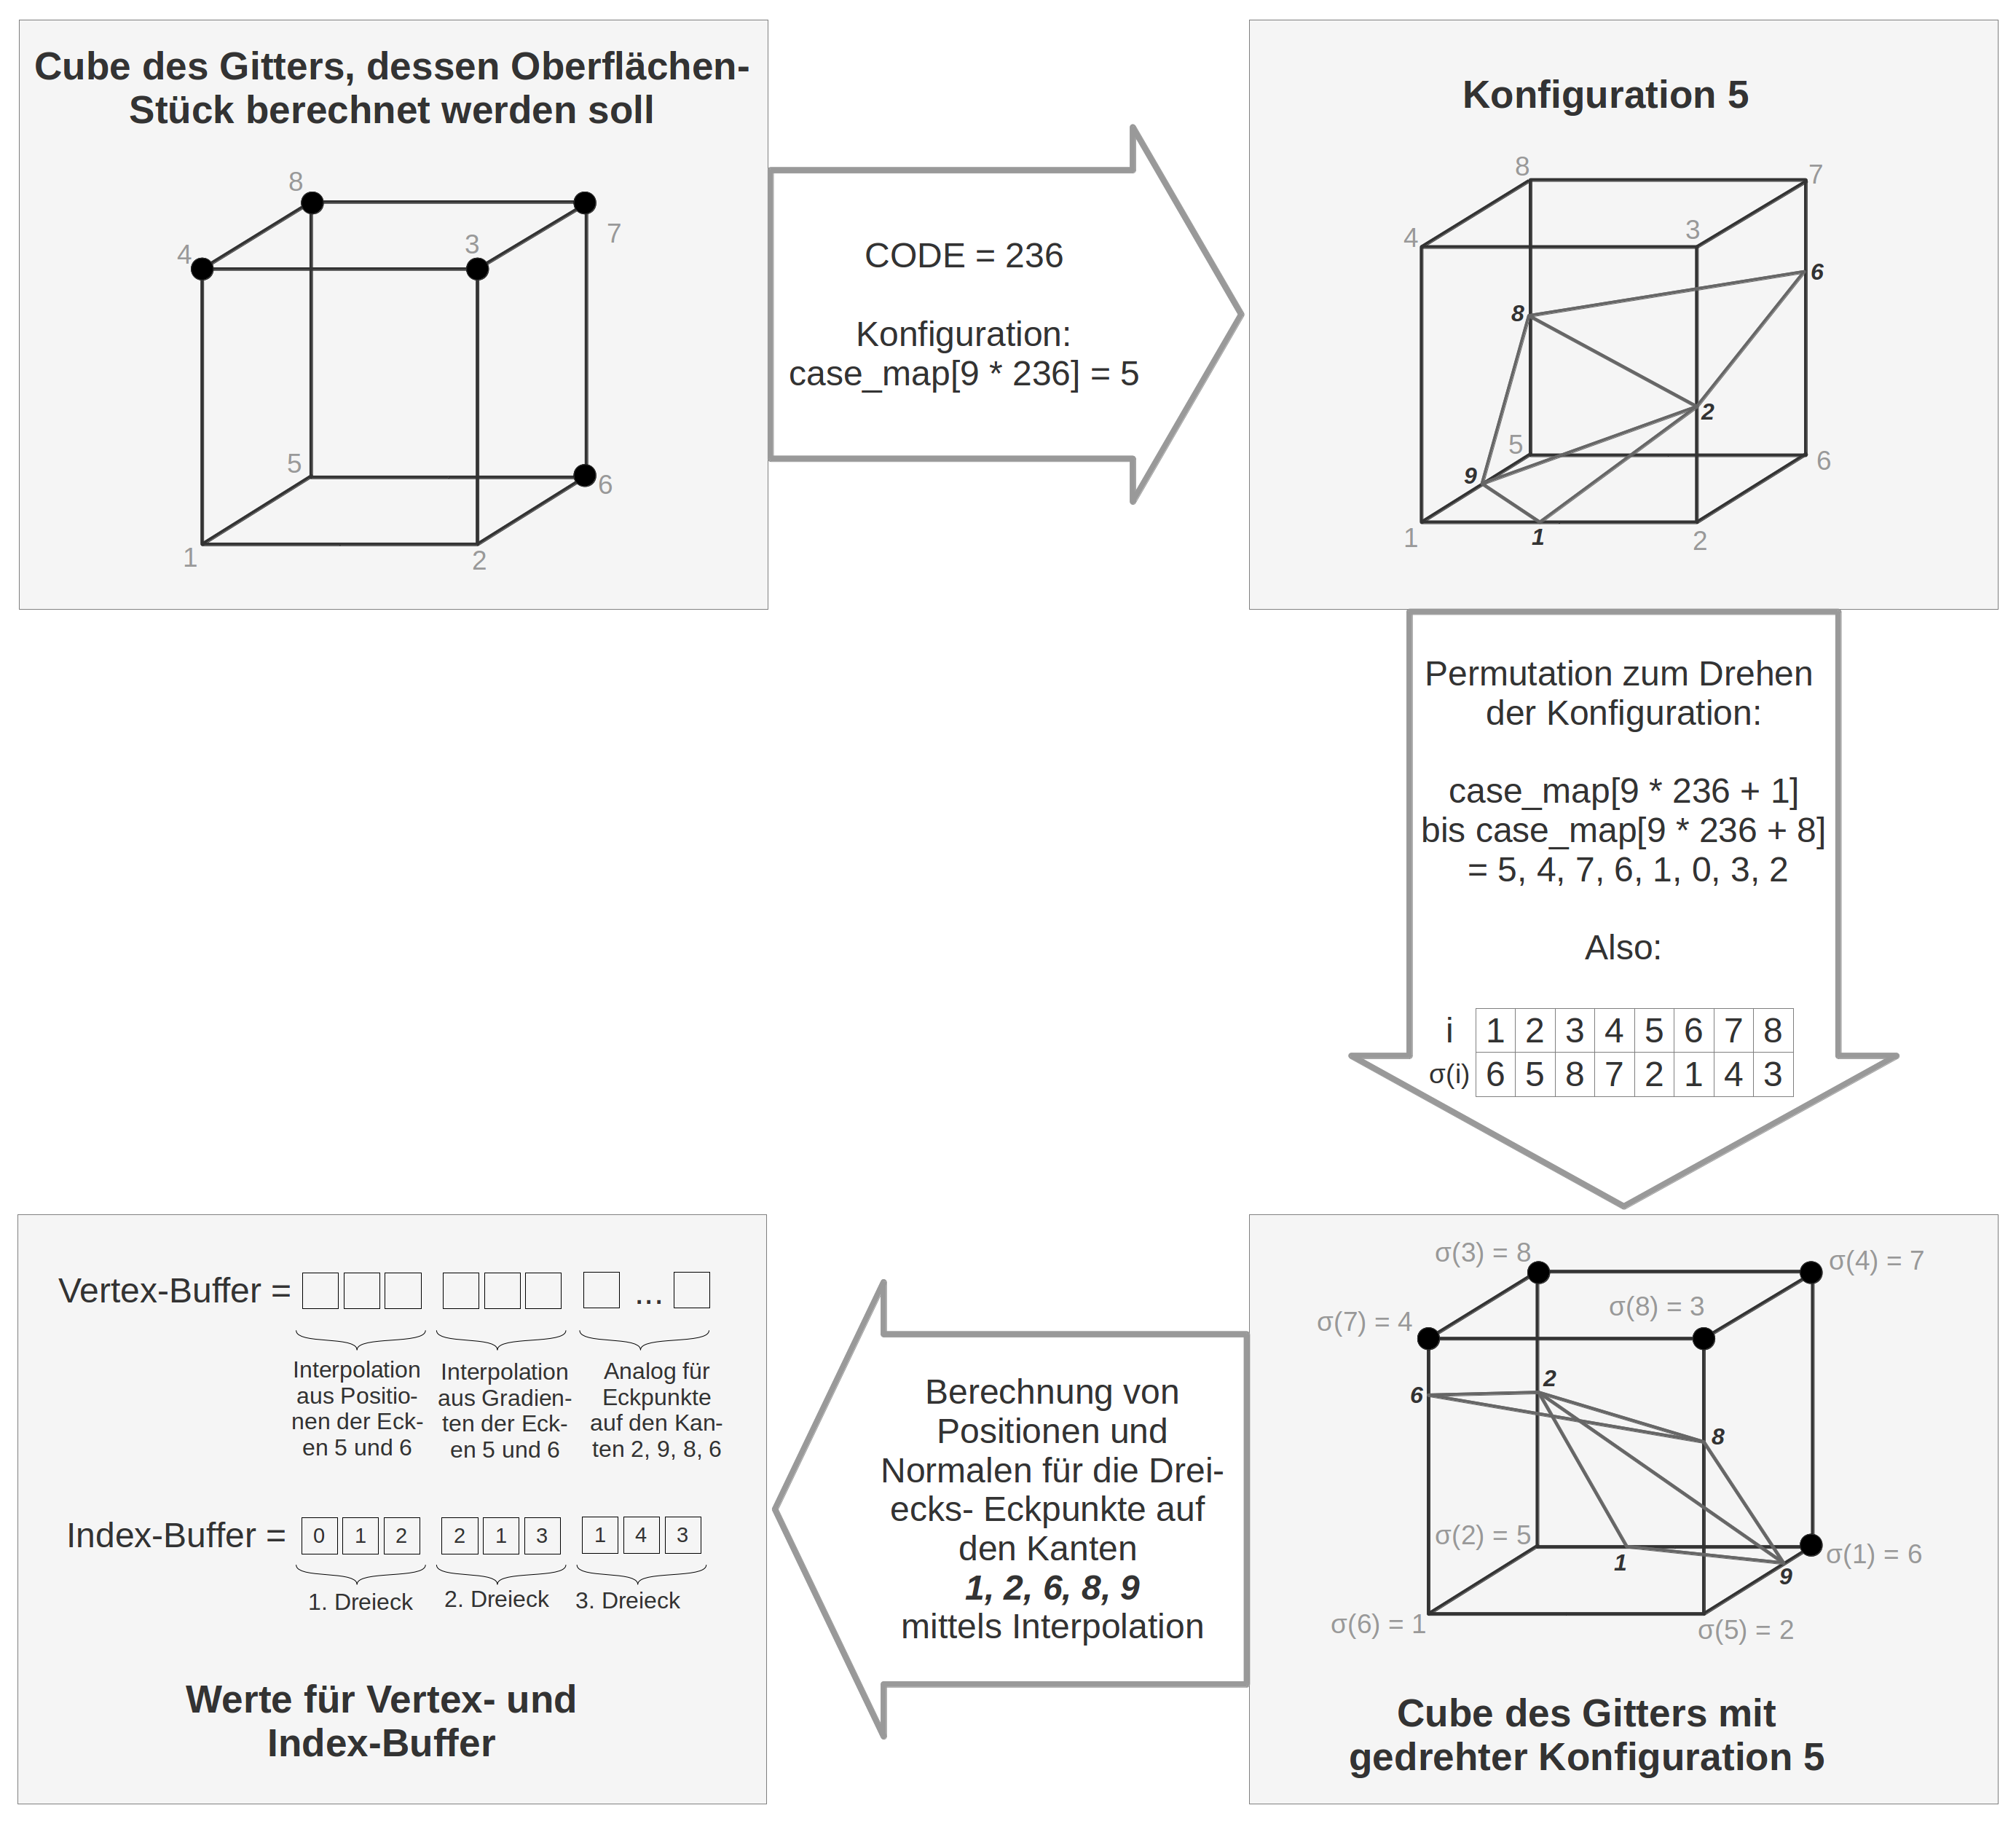
\includegraphics[scale=0.2]{images/Cube-Ablauf}
\end{center}
